\documentclass{article}
\usepackage[utf8]{inputenc}
\usepackage{tipa}
\usepackage{tikz}
\usepackage{tikz-qtree}
\usepackage{phonrule}
\usepackage{fullpage}
\usepackage{pgf-pie}

\title{\LaTeX homework}
\author{Celina Czyszczon }
\date{May 2019}

\begin{document}

\maketitle

\section{Favourite topis in linguistics}
\begin{enumerate}
    \item neurolinguistics 
    \item sociolinguistics 
    \item sentiment analysis 
    \item phonetics
\end{enumerate}
\newline 
\section{Something about me}
\textipa{/"maI "neIm Iz "s@lin@|| "aIm @ "stJU:d@nt @v "nAtSr@l "lANgw@dZ "pr@UsEsIN @t D@ jU:nI"v@rs@ti @v gdańsk || aIm "O:lseU @n "INglIS "tItS@r At "Aksf@rd "lANgw@dZ "sEnt@|| In "maI "fri: "taIm aI "laIk tu "lIs@n tu "mju:zIk @nd "wA:tS "netflIks||/}

\textipa{/"lubiE po"dru\textrtailz \textepsilon  oraz go"towa\textltailn \textepsilon||"mojE ulu"bionE po"travy to "kluski| ro"lada i ka"pusta||/}

\newpage
\section{Syntax tree - 
\small{I told you talking to your boss would be a bad idea.}} 
\begin{tree1}

\newline
\tiny
\qtreecenterfalse

\Tree[.CP [.C' [.C decl. ] [.TP [.NP I ] [.T' [.T past-1p.s. ] [.VP [.V' [.V tell ] [.Np you ] [.CP [.C' [.C decl. ] [.TP [.CP  [.C' [.C decl. ] [.TP [.PRO ] [.T' [.T - ] [.VP [.V' [.V' [.V talking ] ] [.PP [.P' [.P to ] [.NP [.N' [.DP your ] [.N' [.N boss ] ] ] ] ] ] ] ] ] ] ] ] [.T' [.T would ] [.VP [.V' [.V be ] [.DP [.D' [.D a ] [.NP [.N' [.AP bad ] [.N' [.N idea ] ] ] ] ] ] ] ] ] ] ] ] ] ] ] ] ] ]

\end{tree1}

\section{Phonological rules}
\newline
\begin{itemize}
    \item Tapping:
        \newline
        \phonb{/t/}{[\textipa{R}]}{\phonfeat{+vowel}}\phonfeat{+vowel\\ -stress}
    \newline
    \item Spirantization:
        \newline
        \phonl{\phonfeat{+stop \\ -voice}}{\phonfeat{+voice \\-stop \\+fricative}}{\phonfeat{+vowel}}{\phonfeat{+vowel}}
    \newline
    \item Dentalization:
        \newline 
        \phonb{\phonfeat{\textipa{l}}}{[\textipa{\|[\textltilde]}}{}{\textipa{T}}
    \newline
\end{itemize}

\section{NLP equation}
\newline
Equation from the article \textit{Sentiment Analysis and Subjectivity} by Bing Liu
\newline
\newline

\begin{math}
oo(phrase) = log_2 \left(\frac{hits(phraseNEAR 'excellent')hits('poor')}{hits(phraseNEAR 'poor')hits('excellent')}\right)
\end{math}

\newpage
\section{Drawing Pie Charts with \texttt{pgf-pie}}

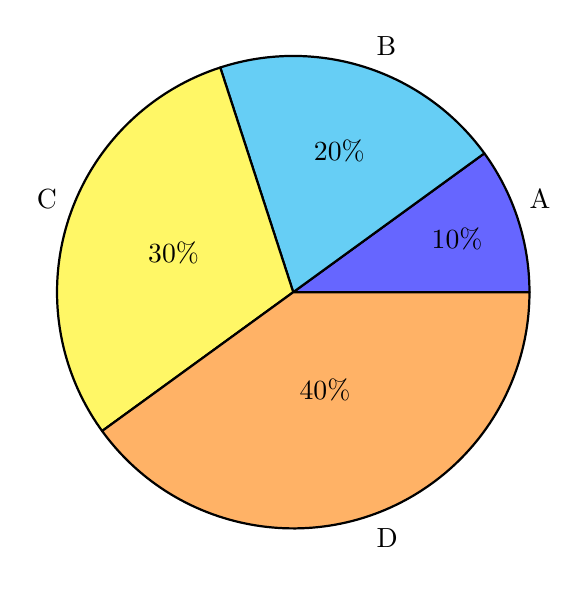
\begin{tikzpicture}
\pie{10/A, 20/B, 30/C, 40/D}
\end{tikzpicture}

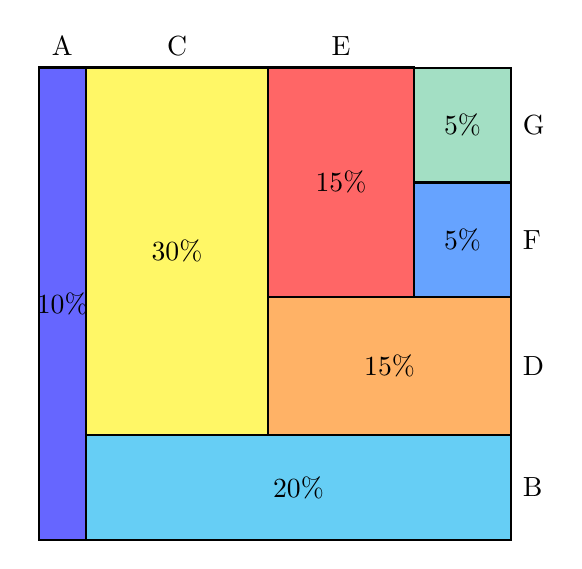
\begin{tikzpicture}
  \pie[square]{10/A, 20/B, 30/C, 15/D, 15/E, 5/F, 5/G}
\end{tikzpicture}

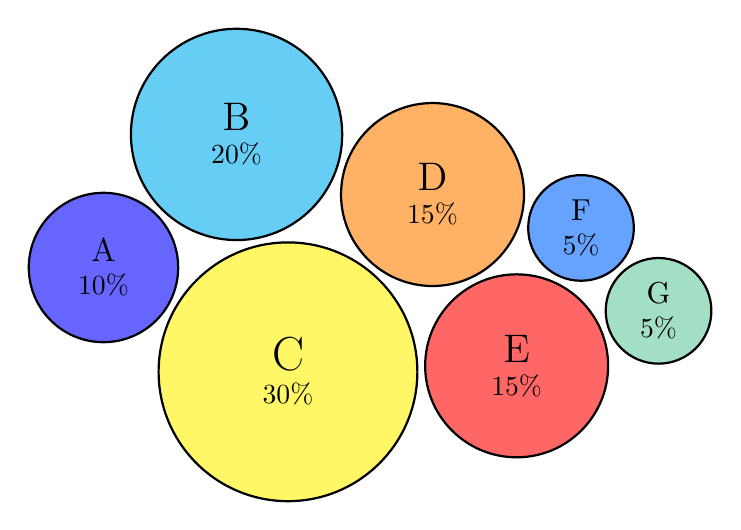
\begin{tikzpicture}
  \pie[cloud, text=inside, scale font]{10/A, 20/B, 30/C, 15/D, 15/E, 5/F, 5/G}
\end{tikzpicture}

\end{document}

